\section{Исследовательский раздел}

Программное обеспечение реализовано на дистрибутиве Ubuntu 24.04 LTS Linux, версия ядра 6.8.0-52-generic.

На рисунке \ref{img:sys1} представлены записи из системного журнала в результате инициализации разработанного драйвера.

\begin{figure}[!htb]\centering
	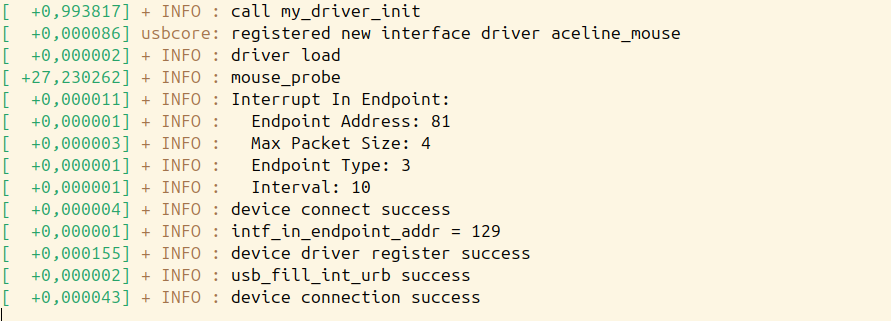
\includegraphics[width=0.9\textwidth]{../img/sys1.png}
	\caption{Инициализация разработанного драйвера}
	\label{img:sys1}
\end{figure}

На рисунке \ref{img:sys2} представлены записи из системного журнала в результате запуска разработанного демона.

\begin{figure}[!htb]\centering
	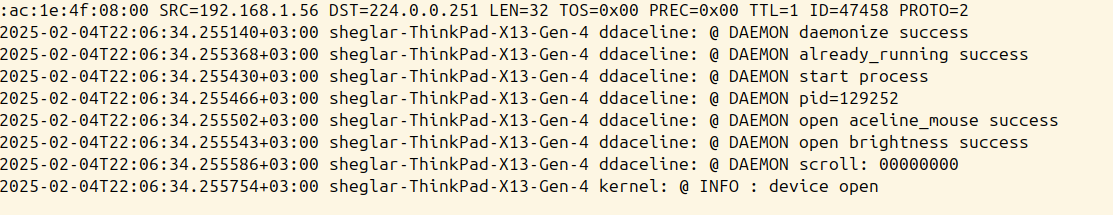
\includegraphics[width=0.9\textwidth]{../img/sys2.png}
	\caption{Запуск разработанного демона}
	\label{img:sys2}
\end{figure}

На рисунках \ref{img:sys3}, \ref{img:sys4} представлены записи из системного журнала в результате прокрутки колесика мыши и нажатия кнопок соответственно.

\begin{figure}[!htb]\centering
	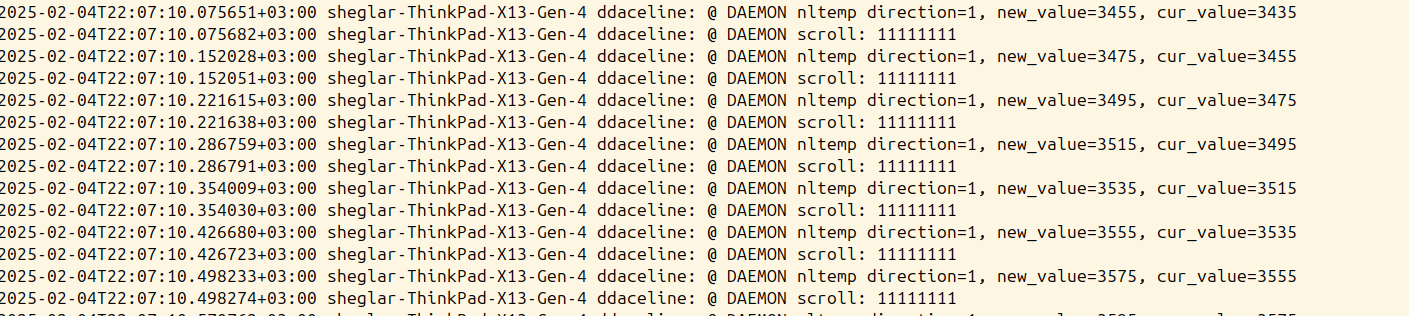
\includegraphics[width=0.9\textwidth]{../img/sys3.png}
	\caption{Прокрутка колесика мыши}
	\label{img:sys3}
\end{figure}

\begin{figure}[!htb]\centering
	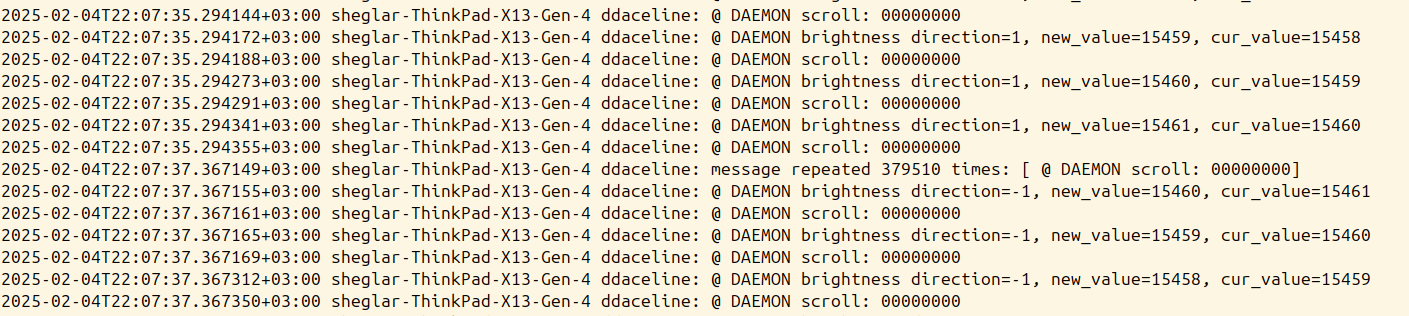
\includegraphics[width=0.9\textwidth]{../img/sys4.png}
	\caption{Нажатие кнопок мыши}
	\label{img:sys4}
\end{figure}

На рисунке \ref{img:sys5} представлены записи из системного журнала в результате завершения разработанного драйвера.

\begin{figure}[!htb]\centering
	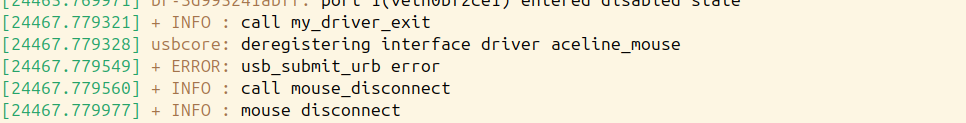
\includegraphics[width=0.9\textwidth]{../img/sys5.png}
	\caption{Завершение разработанного драйвера}
	\label{img:sys5}
\end{figure}
